\directlua{pdf.setminorversion(4)}

\documentclass{standalone}
\usepackage{tikz}
\usepackage{tikz-feynman}

\begin{document}

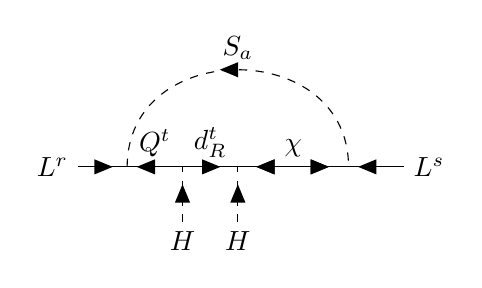
\begin{tikzpicture}
  \begin{feynman}
    \vertex (A) {$L^{r}$};
    \vertex [right=2.7em of A] (B);
    \vertex [right=2em of B] (C);
    \vertex [right=2em of C] (D);
    \vertex [right=4em of D] (E);
    \vertex [right=2em of E] (F) {$L^{s}$};
    \vertex [below=2em of C] (G) {$H$};
    \vertex [below=2em of D] (H) {$H$};
    \diagram* {
      (A) -- [fermion] (B) -- [anti fermion, edge label=$Q^{t}$] (C) -- [fermion, edge label=$d_{R}^{t}$] (D) -- [anti majorana, edge label=$\chi$] (E) -- [anti fermion] (F),
      (B) -- [anti charged scalar, half left, edge label=$S_{a}$] (E),
      (G) -- [charged scalar] (C),
      (H) -- [charged scalar] (D),
    };
  \end{feynman}
\end{tikzpicture}

\end{document}
